\begin{figure*}[t!]
  \centering
   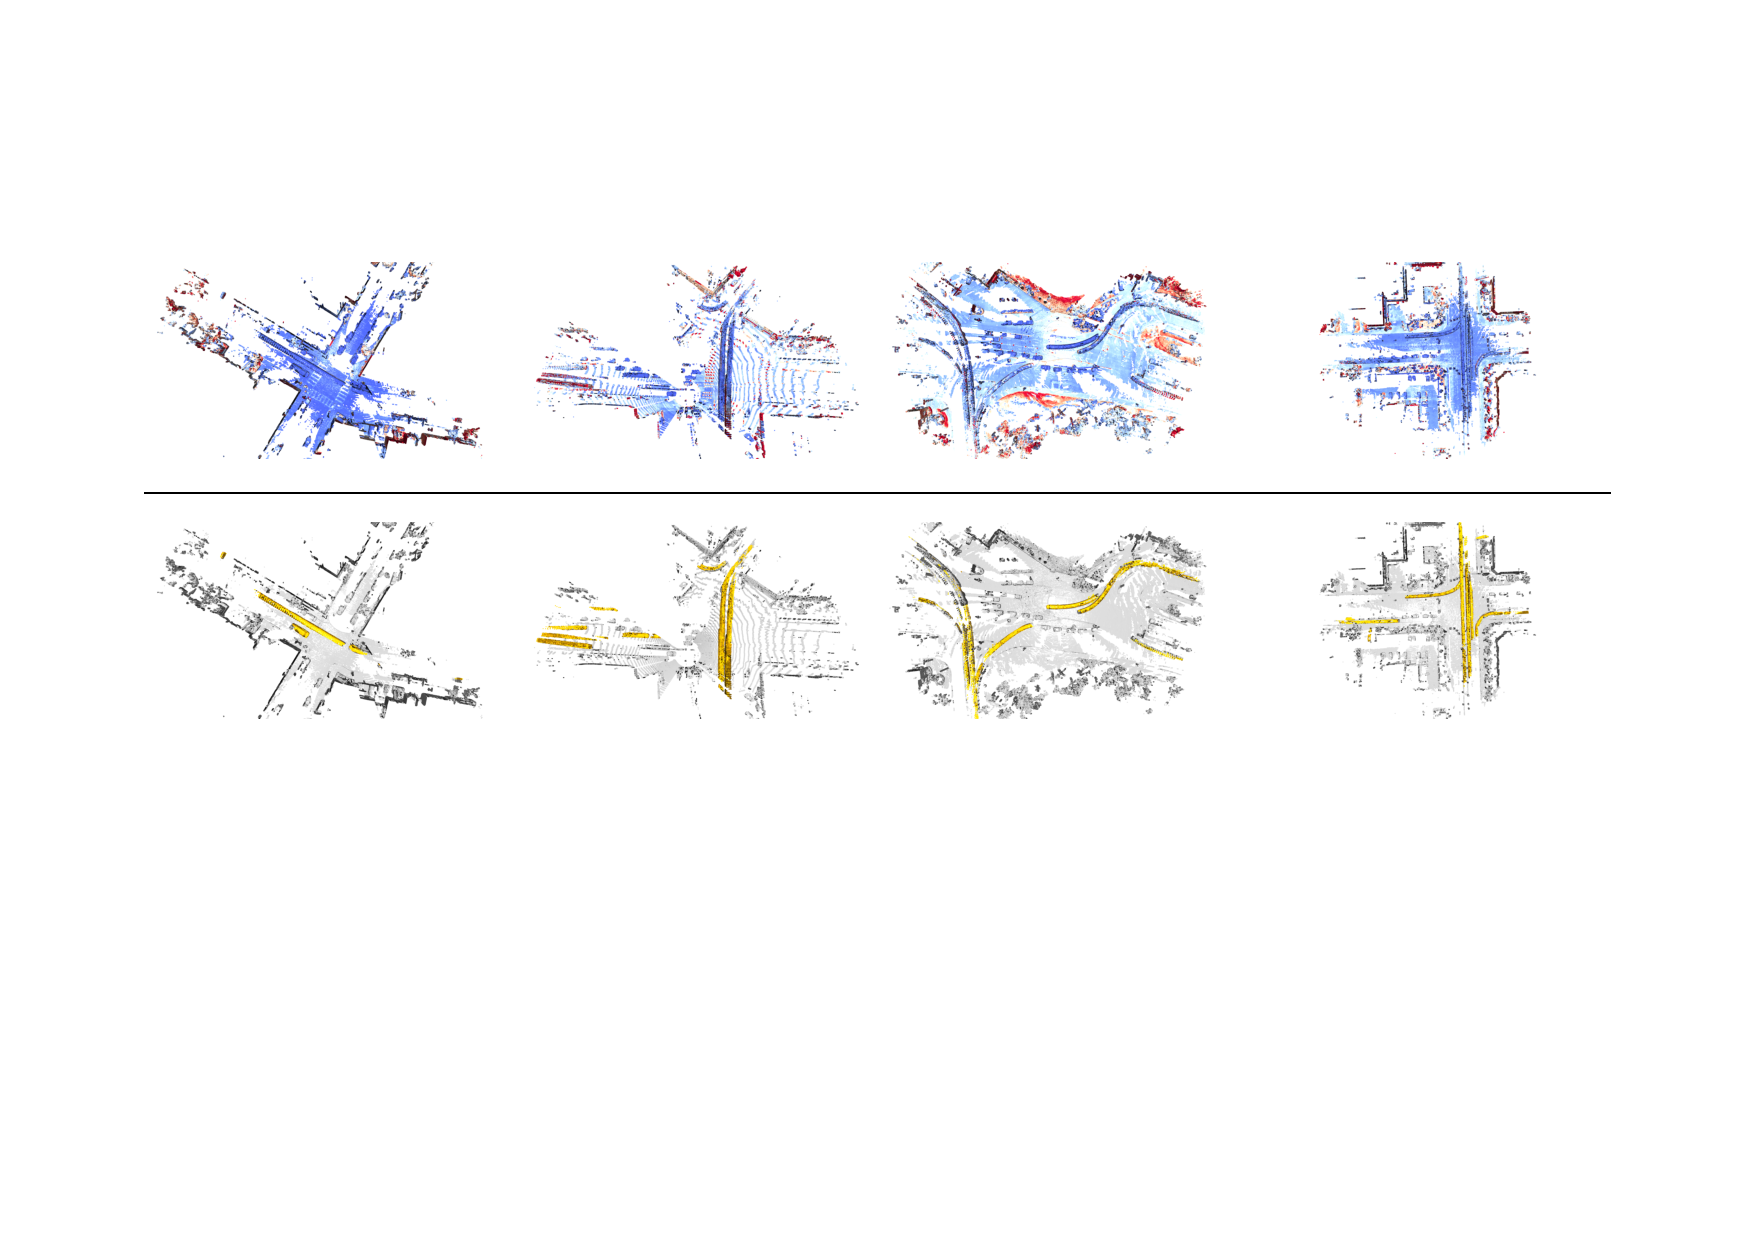
\includegraphics[width=1\columnwidth]{Figures_sup/4_scenes_sup.pdf}
   \caption{Visualization of 4 selected scenes from \textit{Waymo Dynamic} dataset. For each scene, we aggregate 50 frames. In the first row, points are color-coded by the intensity values(0 ~\bwrDyNFL~ 0.25). In the second row, dynamic vehicles are painted as \textcolor{yellow}{yellow}.}
   \label{fig:4_scenes_supp}
\end{figure*}

\begin{figure*}[t!]
  \centering
   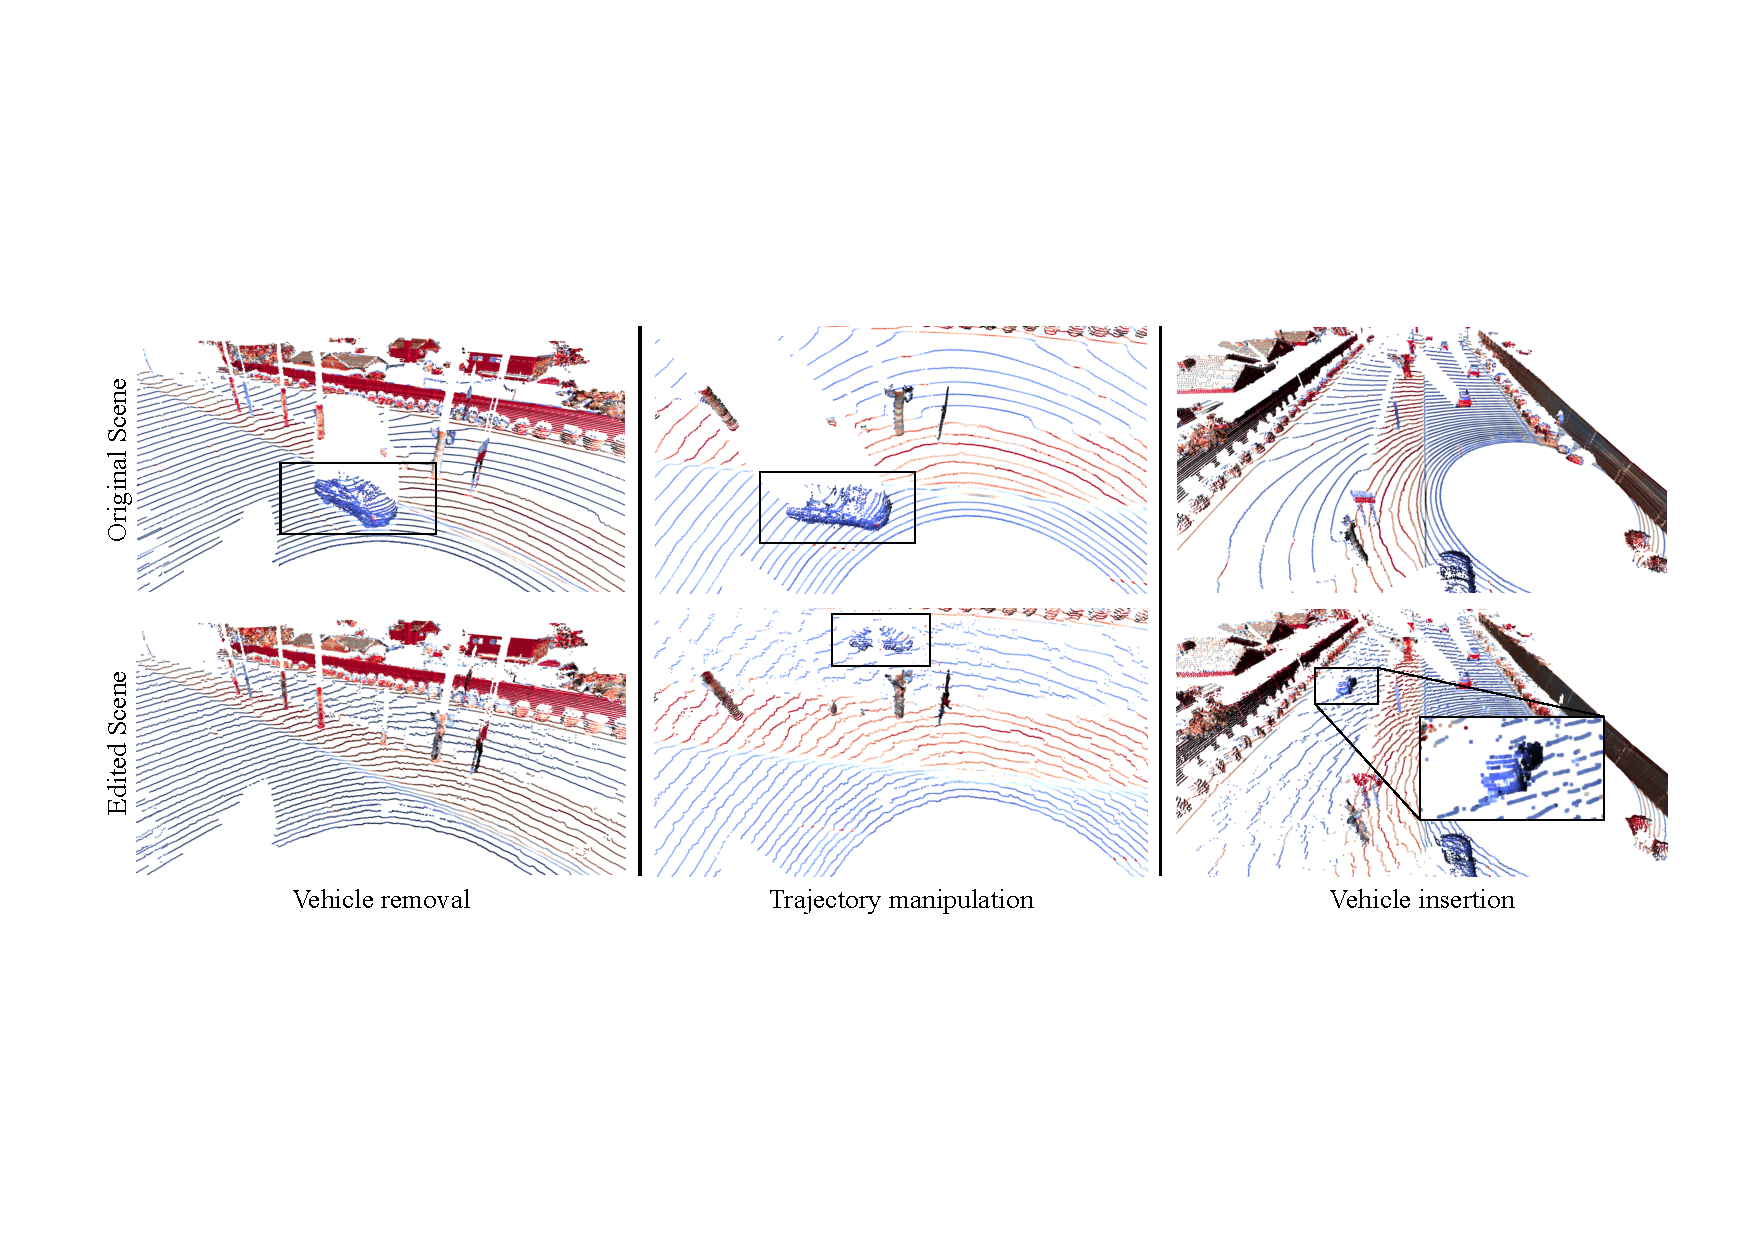
\includegraphics[width=1\columnwidth]{Figures_sup/supp_scene_edit.pdf}
   \caption{Visualization of scene editing capabilities. We showcase 3 kinds of scene editing capabilities including vehicle removal(left), trajectory manipulation(middle) and vehicle insertion(right). The first row represents the original scenes, the second row demonstrates the scenes after editing. All points are color-coded by the intensity values(0 ~\bwrDyNFL~ 0.25).}
   \label{fig:scene_editing_supp}
\end{figure*}

\section{More qualitative results}\label{sec:sup_visual}
In this section, we provide more qualitative results. In \cref{fig:4_scenes_supp}, we showcase the 4 scenes from \textit{Waymo dynamic} dataset. We show additional scene editing results in~\cref{fig:scene_editing_supp}. Please check the supplementary videos for more qualitative results.
